\chapter{Queries}

After the insertion of all available data into the HBase cluster, we implemented several queries over the tables of 'friends' and 'check-ins'. 
These queries can be imposed to any 
social networking service that contains data about users that check in to several locations and have as friends other users of the service. 
As HBase is a NoSQL database and doesn't have a query execution language like SQL for example, 
the implementation of the queries was done using HBase coprocessors. In this way the computation of intermediate results and other complex calculations is 
transfered to the region servers that contain the respective data, decongesting the client from a heavy computational load.

\section{Query implementation}

We implemented the following queries over the data of tables 'friends' and 'check-ins' using HBase coprocessors. 

\subsection{Most visited POI query}

This query contains the following question to the available data:
\begin{center}
 "Get the most visited points of interest of a certain user's friends"
\end{center}

The query is implemented in the following steps:

\begin{enumerate}
 \item The client calls the coprocessor that returns the friends of the specified user. The coprocessor runs on the region server that contains 
 the row of the table 'friends' that has as key the user id of the desired user. The client receives back a list of user id's that 
 represent his friends.
 \item The client splits the list of friends into sections according to the initial split of the 'check-ins' table into 32 regions. In this way, 
 each splitted friends list will contain row keys that belong to only one region server.
 \item The client issues a call to the coprocessor that calculates the most visited POIs for every splitted friend list. 
 More specifically, the client starts a new thread that is responsible for calling the coprocessor and getting the result back. 
 In this way, the client issues parallel calls to the coprocessor and the calculations to the respective region servers are done simultaneously.
 \item The coprocessor that runs on each region server gets from the 'check-ins' table the rows that include all the check-ins of the user friends 
 that are assigned to this region. He then iterates over each row in order to store and count how many times the user's friend has visited each POI. 
 The POIs are stored into a hash table for faster calculations. At the end, he iterates over the hash table in order to get the POI that the 
 specific friend visited the most times.
 \item Finally, the client merges the results that he got back from each coprocessor call and forms the final result, which contains the place and how many times 
 each of his friends went to their most visited POI.
\end{enumerate}

\subsection{News Feed query}

This query contains the following question to the available data:
\begin{center}
 "Get the check-ins of all the friends of a specific user for a certain day into chronological order"
\end{center}

The query is implemented in the following steps:

\begin{enumerate}
 \item The client calls the coprocessor that returns the friends of the specified user. The coprocessor runs on the region server that contains 
 the row of the table 'friends' that has as key the user id of the desired user. The client receives back a list of user id's that 
 represent his friends.
 \item The client splits the list of friends into sections according to the initial split of the 'check-ins' table into 32 regions. In this way, 
 each splitted friends list will contain row keys that belong to only one region server.
 \item The client issues a call to the coprocessor that calculates the news feed for every splitted friend list. 
 More specifically, the client starts a new thread that is responsible for calling the coprocessor and getting the result back. 
 In this way, the client issues parallel calls to the coprocessor and the calculations to the respective region servers are done simultaneously.
 \item The coprocessor that runs on each region server gets from the 'check-ins' table the rows that have as key the friend's ids. Moreover, 
 there are certain columns that are selected from each row. These are the ones that are between two certain timestamps, as the columns have 
 as qualifiers the timestamp of the check-in. The start timestamp is the one that corresponds to the UTC timestamp conversion of the start of the 
 specific day at 12 am and the end timestamp corresponds to the end of the day at 12 am of the next day. In this way, the coprocessor returns 
 only the check-ins of every friend that were made the intended day.
 \item The client merges the the resuls that he got back from the multiple coprocessor calls into one list of user check-ins. Finally, 
 the client sorts this list in order to present the check-ins of the user's friends into chronological order.
\end{enumerate}

\subsection{Correlated Most Visited POI query}

This query contains the following question to the available data:
\begin{center}
 "Get the number of times that a user's friends have visited the user's most visited POI"
\end{center}

The query is implemented in the following steps:

\begin{enumerate}
 \item The client calls the coprocessor that returns the friends of the specified user. The coprocessor runs on the region server that contains 
 the row of the table 'friends' that has as key the user id of the desired user. The client receives back a list of user id's that 
 represent his friends.
 \item The client splits the list of friends into sections according to the initial split of the 'check-ins' table into 32 regions. In this way, 
 each splitted friends list will contain row keys that belong to only one region server.
 \item The client calls the most visited POI coprocessor in order to get the most visited POI of the specific user.
 \item The client issues a call to the coprocessor that calculates the correlated most visited POI for every splitted friend list. 
 More specifically, the client starts a new thread that is responsible for calling the coprocessor and getting the result back. 
 In this way, the client issues parallel calls to the coprocessor and the calculations to the respective region servers are done simultaneously.
 \item The coprocessor that runs on each region server gets from the 'check-ins' table the rows with the check-ins of all the friends that are 
 on that region. Then he iterates over every check-in and checks whether it's location is the same with the location of the most visited POI 
 of the original user. In this way it counts how many times each friend went to that place and returns that counter as a result.
 \item The client merges the resuls that he got back from the multiple coprocessor calls and presents to the user which friends of him went 
 to his most visited POI and how many times they visited that place.
 \end{enumerate}

\section{Queries execution}

\subsection{Workload}

Using the above queries we created a workload in order to test the behavior of the HBase cluster to multiple requests. More specifically, the workload 
consists of the three different type of queries, since they all refer to the same HBase tables. Moreover, the workload takes as input the number of queries 
that will be executed. In addition, since all queries include the retrieval of the friends of one user, that user is chosen randomly. The user that 
corresponds to each query is chosen using a generator of random numbers that follows a uniform distribution. 
The range of this distribution if the total number of available users, which is 9464.

Then, according to the number of queries, all types of queries participate in the workload in a cyclic assignment. 
For example, if the client wants 5 queries to be executed then those will be 1. most visited POI, 2. news feed, 3. corellated most visited POI, 
4. most visited POI, 5. news feed. Also, the queries are executed in parallel as different threads. In this way, the HBase cluster 
receives simultaneously the query requests. The total execution time of the 
workload will be the biggest execution time amongst the queries of the workload. 

\subsection{Workload generation setup}

There is one client that according to the specified number of queries to be executed, creates the workload in the way described previously. This client is hosted 
on a VM with 2 CPU, 4 GB RAM and 40 GB disk. The client is responsible to receive the number of queries to be executed and create the workload in the way 
described previously. The queries arrive at the same time in the HBase cluster that was described in section 4.1.

The workload is executed in the following setup:

\begin{figure}[H]
  \centering
  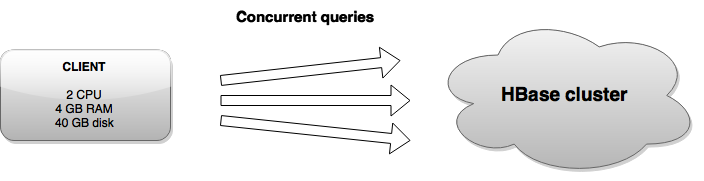
\includegraphics[width=0.8\textwidth]{figures/query_ex_gray.png}
  \caption{Query execution architecture}
\end{figure}

\subsection{Scalability testing}

Using the above architecture we performed a scalability testing, in order to evaluate how HBase handles the above workload for the specified dataset storage model 
in different cluster sizes. We calculated the latency and throughput of the system. More specifically, latency is the mean 
execution time of the queries. Throughput is the number of queries executed per second. 

\[latency = \frac{\text{total execution time of all queries}}{\text{number of queries}} sec\]
\[throughput = \frac{\text{number of queries}}{\text{maximum query execution time}} queries/sec\]

We calculated the latency and throughput of the system for an increasing number of concurrent queries. We started with the HBase cluster having 32 nodes, as 
described previously. Then, we resized the cluster to 24, 16, 8 and 4 nodes in order to observer the variations in the latency and throughput. 
The restructure of the cluster was achieved by decommissioning the datanodes and region servers to the desired number. Both HDFS and HBase offer 
commands in order to achieve the resize of the cluster by moving data and regions into the remaining nodes, preventing data loss and ensuring that the 
regions will be data balanced. 

The scalability testing can be presented in the following tables and corresponding plots:

\begin{table}[H]
\begin{center}
\begin{tabular}{|c|c|c|c|c|c|}
\hline
Queries no. & 32 nodes & 24 nodes & 16 nodes & 8 nodes & 4 nodes \\ \hline
5 & 2.4   & 2.8    & 2.4   & 2.6   & 3\\ \hline
10 & 2.5  & 2.7    & 2.7   & 3.2   & 4.6\\ \hline
15 & 3.2  & 3.06   & 3.6   & 3.73  & 5\\ \hline
20 & 3.4  & 3.9    & 4.2   & 4     & 5.95\\ \hline
25 & 5    & 5.32   & 5.56  & 5.76  & 6.56\\ \hline
30 & 5.5  & 5.76   & 6.36  & 6.03  & 7.66\\ \hline
35 & 6.37 & 6.08   & 7.06  & 7.51  & 9.91 \\ \hline
40 & 6.97 & 7.52   & 8.05  & 8.35  & 10.725 \\ \hline
45 & 7.55 & 8.31   & 9.02  & 10    & 10.86 \\ \hline
50 & 8.34 & 9.02   & 10.32 & 11.2  & 13.6 \\ \hline
55 & 8.96 & 10.14  & 11.21 & 11.45 & 13.85 \\ \hline
60 & 10.26 & 10.88 & 11.3  & 12.58 & 15.98 \\ \hline
\end{tabular}
\end{center}
\caption{Scalability testing - Latency}
\end{table}


The latency increases as the number of nodes of the HBase cluster decreases. Latency is the mean execution time of the queries. Thus, 
it is expected that the latency will increase when there are fewer nodes in the cluster. In more details, when the cluster size reduces there are fewer servers to 
handle the read requests and calculations that accompany the query. Therefore, the remaining HBase region servers have to handle more workload as opposed to when 
the cluster size was bigger. More specifically, since the data on the tables 'friends' and 'check-ins' are splitted into 32 regions in order to be equally 
distributed in the 32 nodes cluster, when we reduce the nodes, a region server can end up with more than one region from each table. In this way, the region 
server will have to handle more coprocessor calls as he has to server calculations for more data than before. Consequently, the execution time of the queries 
increases as there are fewer region servers and datanodes. Additionally, the latency increases as the client sends more concurrent queries. This happens due to the fact 
that as the number of concurrent queries elevate the servers cannot resolve them simultaneously and many of them have to wait in the servers queues. Therefore, 
there are queries that have additional waiting time to their total execution time. This waiting time becomes bigger when there are fewer servers to handle the 
concurrent queries. On the same level, when there is a small number of concurrent queries on different cluster sizes, then the latency is approximately the same 
due to the fact that there is no added waiting time. 

\begin{figure}[H]
  \centering
  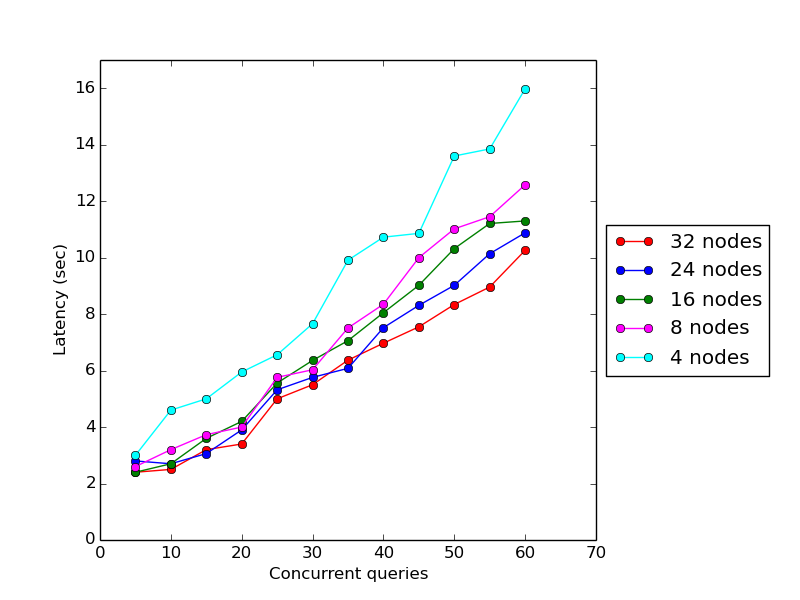
\includegraphics[height=0.6\textwidth]{figures/scalability_latency.png}
  \caption{Scalability testing - Latency}
\end{figure}

\begin{table}[H]
\begin{center}
\begin{tabular}{|c|c|c|c|c|c|}
\hline
Queries no. & 32 nodes & 24 nodes & 16 nodes & 8 nodes & 4 nodes \\ \hline
5 & 1.66   & 1.66  & 1.66 & 1.66 & 1.25\\ \hline
10 & 3.33  & 2.5   & 2    & 1.8  & 1.66\\ \hline
15 & 3.75  & 3.45  & 3.2  & 2.9  & 2.54\\ \hline
20 & 4     & 3.9   & 3.5  & 3    & 2.5\\ \hline
25 & 4.46  & 3.77  & 3.46 & 3.47 & 2.77\\ \hline
30 & 5     & 4.28  & 3.75 & 3.33 & 2.72\\ \hline
35 & 5     & 4.375 & 3.9  & 3.78 & 2.6 \\ \hline
40 & 5.2   & 4.44  & 4    & 3.63 & 2.85 \\ \hline
45 & 5.425 & 4.5   & 4.09 & 3.75 & 2.8125 \\ \hline
50 & 5.55  & 4.54  & 4.16 & 3.84 & 2.63 \\ \hline
55 & 5.5   & 4.58  & 4.13 & 3.66 & 2.65 \\ \hline
60 & 5.2   & 4.61  & 4    & 3.52 & 2.72 \\ \hline
\end{tabular}
\end{center}
\caption{Scalability testing - Throughput}
\end{table}

Throughput is the number of queries executed per second. It is indicative of the performance of the system. For the current setup and workload, we observe that 
the throughput increases as the size of the cluster becomes bigger. This is expected due to the fact that more servers can serve more concurrent queries. 
When the number of servers increases the amount of work assigned to each server reduces, if the cluster is balanced. In our case, we ensure that the cluster 
is balanced as far as the data are concerned, when we pre-split the data into 32 regions. Also, HBase runs a balancer that keeps the regions equally 
distributed to the region servers. Therefore, when the cluster has 32 region servers, those have to run calculations over fewer data when the coprocessors are 
called, as opposed to when the cluster has fewer nodes. Moreover, we can see that for a specific cluster size the throughput increases as the number of 
concurrent queries elevate. This indicates that the system can handle a bigger load without dropping in performance. However, there is a certain limit to the 
throughput that prevents it from increasing even more. In every real time system exists that limit and indicates that the system cannot handle more queries per 
second for the specific cluster size. This limit is different according to the number of nodes, while a bigger cluster size can have bigger throughput. 
Finally, we can see that this limit in the throughput is not a fixed value for every cluster size. This is due to the fact that the workload is not preset and 
can variate according to the randomly selected user factor. Additionally, cache affects tremendously the performance. When data for a query are retrieved from 
the server's cache, then the response time is noticeably less than getting the data from the datanode's disk. Also, the workload is executed on a real time system, 
on a cluster of virtual machines whose performance can be affected by the rest users of the cloud service that accomodates the VMs. However, those variations to the 
maximum value of the throughput are small and don't prevent us from seeing a stable limitation to the system's throughput.

\begin{figure}[H]
  \centering
  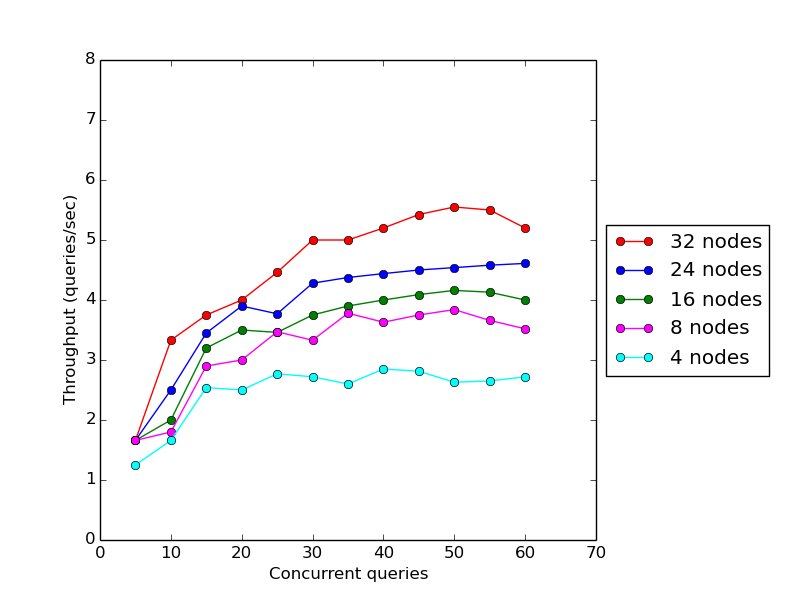
\includegraphics[height=0.6\textwidth]{figures/scalability_throughput.png}
  \caption{Scalability testing - Throughput}
\end{figure}

In conclusion, the HBase cluster that contains the social networking data produced by the generator and stored with the data model described previously, is 
scalable as it has the expected behavior of common scalable systems. 
The construction and execution of the workload that contains the three types of queries, allows as to test the scalability of the HBase cluster 
by calculating the latency and throughput. 





